\documentclass[a4paper, 11pt]{book}

%packages
\usepackage{color} %color-package for text
\usepackage{mhchem} %nuclear notation package
\usepackage[english]{babel} %english language package
\usepackage{amsmath} %math-mode package
\usepackage{wasysym} %astrological symbols package
\usepackage{ifthen} %logical operations for new commands
\usepackage{graphicx}
\usepackage{placeins} %Use for floatbarrier-function
%commands
\newcommand{\comment}[1]{ {\color{red}#1} }
\newcommand{\importantcomment}[1]{ {\Huge \comment{#1}} }

%Packages and styles
\usepackage{natbib}
\bibliographystyle{../references/apj}

%Citation commands
\newcommand\araa{ARA\&A}
\newcommand\aaps{A\&AS}
\newcommand\apj{ApJ}
\newcommand\mycite[1]{{\footnotesize \it \citep{#1}}}

\newcommand{\isotope}[3]{{\footnotesize\ce{^{#3}_{#2}{#1}}}}
\newcommand{\eu}[1]{\isotope{Eu}{63}{#1}}
\newcommand{\re}[1]{\isotope{Re}{75}{#1}}
\newcommand{\os}[1]{\isotope{Os}{76}{#1}}
\renewcommand{\u}[1]{\isotope{U}{92}{#1}}
\newcommand{\pb}[1]{\isotope{Pb}{82}{#1}}
\renewcommand{\th}[1]{\isotope{Th}{90}{#1}}
\newcommand{\w}[1]{\isotope{W}{74}{#1}}
\newcommand{\sos}{Solar system}
\newcommand\betadecay{$\beta^-$-decay }
\newcommand\halflife{
  \ifmmode \tau_{\text{\tiny 1/2}}
  \else $\tau_{\text{\tiny 1/2}}$ \fi
}
\newcommand\msol{
  \ifmmode M_{\astrosun}
  \else $M_{\astrosun}$ \fi
}

\newcommand\omegamodel{\textit{'Omega'}}
\newcommand\eris{\textit{'Eris'}}

\begin{document}

\chapter{Compiling single sections at a time}
For writing purposes only.

%\section{Background}

\subsection{The formation of stars and galaxies}
\subsubsection{Primordial matter}
\subsubsection{Gravitational collapse}
\subsubsection{Galaxies}
\subsubsection{Stars}
\subsection{Nuclear physics of stars}
\subsubsection{The nucleus}
\subsubsection{Interaction of nuclei}
\subsubsection{Production of heavy elements}
\subsection{Galactic chemical evolution}
\subsubsection{More subsections...}

%\section{The \omegamodel\ model}
\label{sec:omega}
\omegamodel\ is a python code developed by Benoit C\^{o}t\'{e} and Christian Ritter\footnote{\url{https://nugrid.github.io/NuPyCEE/}}.
OMEGA stands for 'One-zone Model of the Evolution of Galaxies' and evolves the isotopic content of a galaxy\mycite{cote16a}.
The model is a one-zone model, which means that the entire galaxy is simplified to a single point.
A zero-space-dimensional galaxy model seems unrealistic, but it can be imagined as the mean value for a three-space-dimensional galaxy model.

\begin{figure}
  %Define useful lengths
\newlength{\boxwidth}
\setlength{\boxwidth}{2cm}
\newlength{\boxheight}
\setlength{\boxheight}{1.5cm}
\newlength{\boxdepthx}
\setlength{\boxdepthx}{0.5\boxwidth}
\newlength{\boxdepthy}
\setlength{\boxdepthy}{0.5\boxheight}

%Define useful positions w/short-hand notation
%pos-position, b-bottom, t-top, l-left, r-right, f-front, d-distant
\newcommand\posbfl{(-\boxwidth,-\boxheight)}
\newcommand\posbfr{(\boxwidth,-\boxheight)}
\newcommand\posbdr{(\boxwidth+\boxdepthx,-\boxheight+\boxdepthy)}
\newcommand\posbdl{(-\boxwidth+\boxdepthx,-\boxheight+\boxdepthy)}
\newcommand\postfl{(-\boxwidth,\boxheight)}
\newcommand\postfr{(\boxwidth,\boxheight)}
\newcommand\postdr{(\boxwidth+\boxdepthx,\boxheight+\boxdepthy)}
\newcommand\postdl{(-\boxwidth+\boxdepthx,\boxheight+\boxdepthy)}

\begin{figure}
  \centering
  \begin{tikzpicture}
    %insert galaxy-image in center
    \node (galaxy) at (0.5\boxdepthx,0.5\boxdepthy) {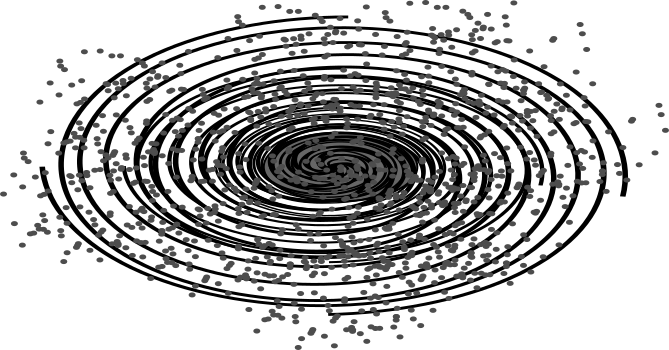
\includegraphics[width=\boxwidth]{galaxy_thumbnail/galaxy.png}};
    %draw bottom plate
    \draw \posbfl -- \posbfr -- \posbdr -- \posbdl -- \posbfl;
    %draw top plate
    \draw \postfl -- \postfr -- \postdr -- \postdl -- \postfl;
    %draw vertical connectors
    \draw \posbfl -- \postfl;
    \draw \posbfr -- \postfr;
    \draw \posbdl -- \postdl;
    \draw \posbdr -- \postdr;
    %add inflow above box
    \draw[thick,->] (0,1.5\boxheight+\boxdepthy) -- (0,1.2\boxheight+\boxdepthy);
    %\draw (-0.5\boxdepthx,2\boxheight) -- (0,2\boxheight-0.5\boxdepthx) -- (0.5\boxdepthx,2\boxheight);
    %\draw (-0.25\boxdepthx,3\boxheight) -- (-0.25\boxdepthx,2\boxheight);
    %\draw (0.25\boxdepthx,3\boxheight) -- (0.25\boxdepthx,2\boxheight);
    \node at (0.6\boxwidth, 1.3\boxheight+\boxdepthy) {\small Primordial gas};
    %add outflow below box
    \draw[thick,->] (0,-1.2\boxheight) -- (0,-1.5\boxheight);
    %\draw (-0.5\boxdepthx,-2\boxheight) -- (0,-2\boxheight-0.5\boxdepthx) -- (0.5\boxdepthx,-2\boxheight);
    %\draw (-0.25\boxdepthx,-1\boxheight) -- (-0.25\boxdepthx,-2\boxheight);
    %\draw (0.25\boxdepthx,-1\boxheight) -- (0.25\boxdepthx,-2\boxheight);
    \node at (0.6\boxwidth, -1.3\boxheight) {\small Enriched gas};
  \end{tikzpicture}
  \caption{\label{tikz:galaxy-iobox}}
\end{figure}

\end{figure}

In this work the \omegamodel\ code will be modified with a wrapper in order to explore various parameters related to nucleosynthesis.

\subsection{Process}
\label{sec:omega-process}
The \omegamodel\ model emulates the chemical evolution of a galaxy starting from the initial primordial gas. A simple stellar population is created by integrating the star formation rate over time.
The star formation rate is calculated either by using a constant star formation rate, the Kennicut-Schmidt law\mycitetwo{fuchs09}{and refernces therein}, or by using an input star formation rate and interpolate over those values.

The stellar populations represent a cluster of stars, with a total mass, initial mass distribution, and initial metallicity distribution.
The initial mass distributions are given as one of the standard distributions, Salpeter, Kroupa, Chabrier, or a power-law, all between some minimum and maximum mass limit (see figure \ref{fig:imf}.
The initial metallicity distribution is the relative mass distribution of isotopes heavier than \isotope{Li}{3}{7}, and the metallicity is the mass fraction of all isotopes heavier than \isotope{Li}{3}{7} combined.
\begin{figure}
  \centering
  \includegraphics[width=\textwidth]{img/various_initial_mass_functions.png}
  \caption{ \label{fig:various-imf}
    A simplified visualization of some of the common initial mass functions in the literature.
    \mycitetwo{cappellari12}{and references therein}, \mycite{salpeter55}, \mycite{kroupa01}, \mycite{chabrier03}, \mycite{miller79}. \\
    image-credit: By JohannesBuchner [CC BY-SA 4.0 (\url{https://creativecommons.org/licenses/by-sa/4.0})], from Wikimedia Commons
  }
\end{figure}


Stellar evolution codes calculate the amount of ejected material, for each isotope, for a star with a given initial metallicity and initial mass. These codes are used to create \textbf{yield tables} for certain kind of stars with different initial mass and metallicity.

In the simple stellar population assumed in the galactic chemical evolution model, these yield tables are used to calculate the chemical composition and mass of ejecta from each group of stars. The ejecta are disspersed back into the interstellar medium (gas of the galaxy model) at delay-times appropriate for each group of stellar mass.
E.g. For a given mass-bin the total mass in stars, number, and age of stars, with initial mass in that bin, are calculated using the total mass of the total stellar mass and mass function chosen. By choosing the yield tables closest in initial mass and initial metallicity the total ejecta composition is calculated and added to the interstellar medium at the age where those stars would have gone supernova.
The material that is not ejected is left as remnants and total mass and number of remnants are also added to the simulation at the time these stars would have gone supernova.

In \omegamodel\ the creation and treatment of simple stellar population is done by another python-program called \texttt{Sygma}.

The \omegamodel\ model is a \textit{one-zone} model, meaning that everything inside the box has been enriched from stellar lifecycles. Everything outside the box is untouched since ``it's creation'', and has the same composition as the material inside the box had to start with.
This composition is called the primordial composition (three parts hydrogen, one part helium and trace amounts of lithium and beryllium), and is derived from the big bang nucleosynthesis (see section\ref{sec:bbn}.
Flow of material can determine the chemical evolution of a galaxy. Enriched material can be ejected from the galaxy by supernova feedback, active galactic nucleus, stellar kick or similar, and non-enriched material can flow into the galaxy.
To describe the chemical evolution of a one-zone model one needs to know the total content of the galaxy (or box) and the distribution. In other words, how much of the total mass is stored as each isotope. Material with the same composition as the box is ejected from the box, and material with another composition falls into the box.

\comment{More on outflow/inflow}

\comment{Insert simple figure here}

\subsection{Uncertainty of parameters}
\comment{uncertainty of parameters and summary of article (cote16a)}

Galaxies consist of many different, widely varying, scales for both spatial and temporal resolution.
The galaxies themselves span hydrodynamical evolution on many kpcs and Gyrs, while their stars and supernovae span scales closer to seconds and meters.
The nuclear processes within stars span nanometer and millisecond timescales, even though stars can last for billion years(with short timescale bursts in between).
Neither analytical/numerical models nor simulations cannot cover all these scales at once, that is when subgrid methods are used. Stellar evolution simulations predict the fate and output from the life of a single star based on sinple input parameters and assumptions of the physical processes that governs the evolution. These solutions are then simplified and applied to more complex galaxy simulations.
Output ejecta from stars are ``looked up in a table'' and applied to the nearby interstellar medium.
All these methods and linked applications introduce some uncertainties and assumptions, both physical and numerical, and these uncertainties are inherited through all methods based on applications of these models. In order to probe how the uncertainties of selected parameters manifest through the resulting galaxy evolution, \mycite{cote16a} presents a simple one-zone, closed-box model of galaxy evolution, called \omegamodel.

%use \figwidth for width of image
\begin{figure}
  \centering
  \includegraphics[width=\figwidth]{img/uncertainty_diagram_cote16a_fig1.png}
  \caption[\mycitetwo{cote16a}{fig.1}]{ \label{img:uncertainty-diagram}
    Qualitative visualization of how uncertainties accumulate in galactic chemical evolution models.
    Experimental data on nuclear reaction rates are uncertain to some degree. The change in rate and uncertainty in stellar conditions are not well known.
    The conditions inside a star of a given mass and metallicity come from 1 dimensional hydrodynamical simulations.
    The combined result from nuclear reactions and hydrodynamical simulations give a stellar models.
    The stellar models are applied to a simple stellar population to account for all the billions of stars in galaxy.
    These stellar models are then applied to a large scale hydrodynamical simulation (like \eris), or a semianalytical galaxy model (like \omegamodel).
    All the steps make assumptions and add uncertainty to the grand total uncertainty that is difficult to map in completeness.

    Diagram is taken from \mycitetwo{cote16a}{fig.1}
  }
\end{figure}


\sygma creates the simplified stellar populations (mass function, total mass, lifetime distribution, initial metallicity).
\omegamodel\ combines several stellar populations to emulate a galaxy evolution.

Stellar yields are tables from stellar evolution simulations.
The tables used in \omegamodel are taken from, among other sources,  NuGrid\footnote{NuGrid collaboration: \href{http://www.astro.keele.ac.uk/nugrid/}{Homepage} \href{https://github.com/nugrid}{Github}} and include AGB stars between 1 and 7 \msol, massive stars between 12 and 25 \msol, all with metallicities at $Z = 0.02, 0.01, 0.006, 0.001, 0.0001$. These tables contain many isotopes between hydrogen and bismuth.

The stellar evolution was calculated with MESA\footnote{MESA is a modular, opensource code to evolve single star systems, and can do so from main sequence to white dwarf stage or core collapse stage. See \href{http://mesa.sourceforge.net}{Homepage} for further information}, post-processing was done with MPPNP \mycite{nugrid08mppnp}, the same nuclear reaction rates were used in all calculations, explosive nucleosynthesis was done with semi-analytical models. Yields are complemeted with SN1a yields from \mycite{sn1aivo13}, \mycite{sn1at03}, \mycite{sn1ai99}, \mycite{sn1at86} and population III yields from \mycite{pop3hw10} (other sources are available from the literature, but these are the focus of the chemical evolution of this thesis. Sources for neutron star mergers will be discussed later).

The probability distribution functions for the input parameters are created from values and uncertainties in the literature.
Methodologically there are, for each input parameter, gathered a list of literature values and uncertainties.
The errors are considered gaussian in nature and distributions are created thereafter,
all the distributions are then averaged to a single distribution.
Then a single gaussian is fitted atop the ``average of gaussians from the literature'',
and the median and standard deviation from
the final fit is used as value and uncertainty for the input parameter in question.

%insert images from cote16a to summarize the parameter-method
\setlength{\subfigwidth}{\linewidth}
\begin{figure}
  \centering
  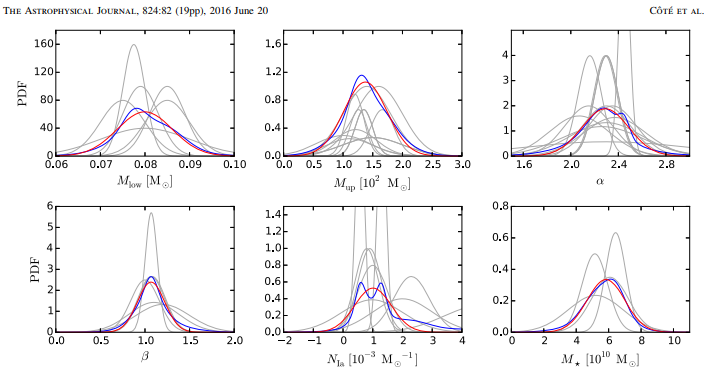
\includegraphics[width=\subfigwidth]{img/parameter_pdfs_cote16a_fig2.png}
  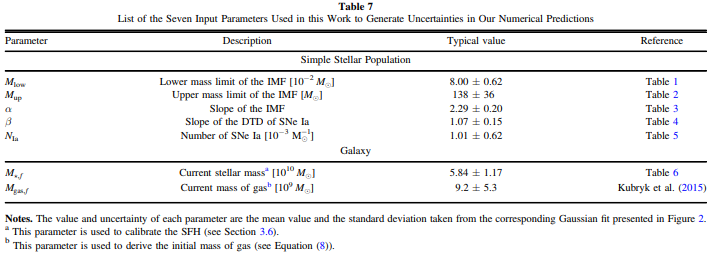
\includegraphics[width=\subfigwidth]{img/parameter_table_cote16a_table7.png}
  \caption{\label{fig:cote16-input-param}
    How the input parameters were determined from multiple sources in the literature. Values and standard deviations averaged to a probaiblity distribution, and then fitted to a single gaussian distribution. Images from \mycitetwo{cote16a}{figure 2 and table 7}.
  }
\end{figure}

\mycite{cote16a} sampled a set calculations, for each parameter in figure \ref{fig:cote16-input-param} a series of 300 calculations were made with a random sampling of the input parameter for the gaussian uncertainty distribution.
A set of 700 calculations were made were all the input parameters were all the input parameters were randomly drawn from their respective gaussian distributions. An additional 300 calculations were made with the final gas-mass and final stellar mass both drawn randomly from their respective gausssian distributions.

Spectroscopic abundance of metals are measured in [X/Y] where X is the metal in question and Y is the reference metal, either plotted against metallicity, [Y/H], or galactic time, Gyr.

The main conclusions are summarized as follows:
\begin{enumerate}
\item{
  The overall uncertainty of spectroscopic metals between 0 and 0.6 dex when plotted against metallicity, but the uncertainty is higher when considered against galactic time.}
\item{
  \begin{itemize}
  \item{Ratio of final mass of gas to final mass of stars affect the uncertianty for early times ([Fe/H] $\lesssim$ -2) since more gas means more hydrogen, while more stars means more iron-production. Since metals are also produced in stars, the ratio does not affect [X/fe] much.}
  \item{Number of type 1a supernovae and their delay time distribution affect the uncertainty of spectroscopic metals at later times([Fe/H] $\gtrsim$ -1.5 $\rightarrow$ t $\gtrsim$ 150Myr), when the delay-time has allowed for type 1a supernovae to occur. Type 1a supernovae add mostly iron to the interstellar medium, while not producing much of metals produced by AGB stars and massive stars. This means that the uncertainty of [X/Fe] will be greatly affected by uncertianties in type 1a supernovae.}
  \item{The high mass slope of the initial mass function, $\alpha$, determines the ratio of massive stars to low-mass stars at all times. Massive stars die quickly and distributed much enriched material into the interstellar medium. Therefor the uncertainty of the slope will always be prevailent in the uncertainty of spectroscopic metals.}
  \item{Uncertainties in the mass ranges of the initial mass function does not affect uncertainties of the spectroscopic abundances much.}
  \end{itemize}
}
\item{
  Uncertainties in the slope of the initial mass function, $\alpha$, and the number of type 1a supernovae affect the uncertainties in the spectroscopic abundances.
  When plotted against metallicity ([Fe/H]) the uncertainty is greatest when the considered metal and the reference metal is not from the same source.
}
\item{
  The characteristics seen from spectroscopic abundance against metallicity is shared regardless of the introduced uncertainties.
  The introduced uncertainties amplify the characterstic shapes, but do not change them. ``Such features are mainly caused by the choice of stellar yields and the type of galaxy considered.''\mycitetwo{cote16a}{p.18}
}
\end{enumerate}

%use \figwidth for width of figure

\begin{figure}
  \centering
  \includegraphics[width=\figwidth]{img/spectroscopic_uncertainties_cote16a_fig6.png}
  \caption[\mycitetwo{cote16a}{fig.6}]{
    \label{img:spectroscopic-uncertainty}
    Spectroscopic abundance of 16 metals relative to iron, considering uncertainties of all parameters (upper bound, lower bound and high mass slope of initial mass function, stellar and gas mass today, number of type 1a supernovae and the slope of the type 1a supernova delay-time distribution).

    Plots and figures are taken from \mycitetwo{cote16a}{fig.6}
  }
\end{figure}

%use \figwidth for width of figure
\centering
\includegraphics[width=\figwidth]{img/age_uncertainties_cote16a_fig11.png}
\caption[\mycitetwo{cote16a}{fig.6}]{
  \label{img:age-uncertainty}
  Uncertainty of spectroscopic abundance of 16 metals relative to iron, considering uncertainties of all parameters (upper bound, lower bound and high mass slope of initial mass function, stellar and gas mass today, number of type 1a supernovae and the slope of the type 1a supernova delay-time distribution).

  Uncertainties relative to mean shown as a function of galactic age.

  Plots and figures are taken from \mycitetwo{cote16a}{fig.6}
}


\FloatBarrier

\subsection{Relevant parameters}
\label{sec:omega-parameters}
\omegamodel\ has many input parameters, both numerical and physical in nature, to guide the evolution of the galaxy. A physical input parameters are model parameters, while a numerical parameter decides on which calculations to choose from and where to get data. E.g initial gas of galaxy is considered physical, while the boolean switch to turn on neutron star mergers are considered numerical

This section will describe the most relevant ones in order of appearance in the program.

\begin{description}
\item[galaxy]
  This string option chooses predefined parameters to best match a certain galaxy on record.
  The relevant options are:
  \begin{description}
  \item[None] No parameters determined.
  \item[milky\_way\_cte] Set present dark matter mass to $10^{12} \msol$ and present stellar mass to $5\times10^{10} \msol$, and use a constant star formation rate of $1 \frac{\msol}{yr}$
  \item[milky\_way] Set present dark matter mass to $10^{12} \msol$ and present stellar mass to $5\times10^{10} \msol$, and use the star formation rate from \mycite{sfrcmr01}
  \end{description}
\item[in\_out\_control] Boolean switch to turn on or off inflow and outflow.
\item[outflow\_rate] \comment{remove this?} Constant outflow rate in $\frac{\msol}{yr}$. Enriched gas from the interstellar medium is removed from the galaxy.
\item[inflow\_rate] Constant inflow rate in $\frac{\msol}{yr}$. Gas with primordial composition \comment{(reference to BBN?)} flows into the galaxy.
\item[mass\_loading] Fraction of solar masses ejected per solar mass created as star. A different way of calculating outflow based on star formation rate.
\item[imf\_type] Which form to use for the initial mass function\comment{explain this somewhere}. 
\item[alphaimf] Slope of lognormal initial mass function. 
\item[sn1a\_rate] This string option chooses which distribution to calculate the rate of type 1a supernovaefrom.
  Options are powerlaw, gaussian, and exponential distribution.
  \begin{description}
  \item[beta\_pow] Set the power of the power law distribution if 'sn1a\_rate' is "power\_law" 
  \item[gauss\_dtd] Set the mean and standard deviation of the gaussian distribution if 'sn1a\_rate' is "gauss" 
  \item[exp\_dtd] Set the e-folding time of the exponential distribution if 'sn1a\_rate' is "exp"
  \end{description}
\item[dt] Length of first timestep (in yrs)
\item[special\_timesteps] Number of logarithmic timesteps
\item[tend] Final point in time (in yrs)
\item[mgal] Initial mass of gas (if not calculated by other means), defaults to $10^{10} \msol$
\item[transitionmass=8]
  Mass-limit that separates the AGB stars from the massive stars\comment{explain these stars somewhere}.
  Defaults to $8\msol$
\item[nb\_nsm\_per\_m] Set the number of neutron star mergers per solar mass formed as stars.
\item[t\_nsm\_coal] Set the time after which all neutron stars collide/merge
\item[table] path to yield table for AGB and massive stars.
\item[sn1a\_on] Boolean switch that turn on or off the use of type 1a supernovae.
\item[nsm\_dtd\_power] Set the powerlaw distribution of the neutron star merger delay-time distribution \comment{explain this somewhere}.
\item[sn1a\_table] Yield table for type 1a supernovae
\item[ns\_merger\_on] Boolean switch to turn on or off binary neutron star mergers
\item[f\_merger] Fraction of binary systems that eventually merge. All systems are considered binary. This is instead of 'nb\_nsm\_per\_m'
\item[m\_ej\_nsm] solar masses ejected per neutron star merger.
\item[nsmerger\_table] Yield table of binary neutron star mergers
\item[bhns\_merger\_on] Boolean switch to turn on or off black hole neutron star mergers
\item[pop3\_table] Yield tables for population III stars
\item[imf\_bdys\_pop3] The boundaries of the initial mass function of population III stars.
\item[nb\_1a\_per\_m] The number of type 1a supernovae per solar mass formed.
  Used to calculate the number of type 1a supernovae from star formation rate.
\item[popIII\_on] Boolean switch that turn on or off the use of Population III stars
\item[out\_follows\_E\_rate] Adds a time-delay to outflow with mass\_loading such that outflow follows supernova rate.
\item[sfh\_array] Two one-dimensional arrays, time and star formation rate, that \omegamodel will interpolate over in order to find the star formation rate at a given time.
\end{description}

\newcommand{\imagefolder}{results/plots_fitting}

\section{Fitting of models}

In order to have the one-zone model \omegamodel\ best reproduce the \eris\ simulation \\
\comment{... continue introduction and description} \\
Some parameters are decidedly locked from the \eris\ simulation directly.
One of the most valuable result from \eris\ (for these purposes)
are the star formation rate thorugh Galactic time (also known as star formation history). The Galctic age in \eris\, is 14Gyr.
In order to produce stars, a mass function has to be set. A mass function is the statistical probability distribution of mass for a population of stars. In \eris\ the Kroupa94
(\comment{insert reference here})\\
(\comment{insert image of distribution here?})
mass function is used, and the same shall also be used for \omegamodel. 
The stellar synthesis in \eris\ postproduction comes from core collapse supernova, type 1a supernova and binary neutron star mergers.
In the appropriate \omegamodel\ the black hole - neutron star mergers shall not be taken into effect,
and the yield table for binary neutron star mergers is chosen to be \comment{insert reference to Arnould} \comment{add comment/description about how the yield table is the r-process from the sun}, because it contains \re{187}.

\comment{define new commands for MWOmega/MWCteOmega/fiducccial model}
\newcommand\mwomega{TEMP-MWOmega}
\newcommand\mwcomega{TEMP-MWcteOmega}
\newcommand\fiduccialomega{TEMP-fiduccial}
\importantcomment{introduce 'our' \omegamodel\ model as the concept \textit{'fiduccial model'}}

\FloatBarrier
\subsection{Inserting parameters directly}
\iffalse
Filenames:
set_sfr_plot_gas_mass.png                
set_sfr_plot_sfr.png                     
set_sfr_plot_spectro.png                 
set_sfr_plot_stellar_mass.png
\fi
\comment{describe parameters: sfr, tend, imf, BNSM/BHNSM, yield-tables etc.}
\comment{fix stellar mass plot data}
The first step towards finding an appropriate parameter space for \omegamodel\ is to make \omegamodel\ follow the stellar evolution of \eris. This is achieved by setting the initial mass function to Kroupa93\comment{(insert reference)}, and the star formation history from the \eris\ simulation. By activating type 1a supernovae and binary neutron star mergers, the stellar evolution of \omegamodel\ should be similar in nature to \eris. In the star formation history of \eris, the endtime is 14Gyr, and the endtime for \omegamodel should be set to the same value. There is only one(out of two) available yield tables for binary neutron star mergers that contain output for \re{187}, in the interest of this project we naturally choose this one\comment{(add reference to yield tables)}.

\begin{figure}[h]
  \centering
  \includegraphics[scale=0.5]{\imagefolder/set_sfr_plot_sfr.png}
  \caption{\label{img:fit-v0-sfr}
    Star formation rate(measured in solar masses of stars formed from gas each year) for four models of \omegamodel\ versus time. 
    \textit{'Eris'} refers to data directly from \eris -simulation. \textit{'Omega' default} refers to the \omegamodel\ model with no change to the initial parameters (see description in section \ref{sec:omega}). \textit{'Omega' MW} refers to the \omegamodel\ model with the Milky Way parameter (see description in section \ref{sec:omega}), and \textit{'Omega' MW cte} refers to the same but with a constant one-solar-mass-per-year star formation rate. \textit{'Omega' w/'Eris'-SFR} refers to the \omegamodel\ model with the star formation and mass function from \eris.
    Firstly it is clear that star-formation is suppressed for all models except \textit{'Omega' default}. This is from the lack of gas to create stars from. Secondly the \textit{'Omega' w/'Eris'-SFR} model is the only model to accurately reproduce the \eris\ star formation at early times. While both \textit{'Omega' MW} and \textit{'Omega' MW cte} are meant to represent the milky way, they cannot be used to accurately represent \eris.
  }
\end{figure}
\begin{figure}[h]
  \centering
  \includegraphics[scale=0.5]{\imagefolder/set_sfr_plot_stellar_mass.png}
  \caption{\label{img:fit-v0-stellarmass}
    Total accumulated stellar mass(cumulutaive sum of stellar mass produces from gas, measured in solar masses) for four models of \omegamodel\ versus time.
    \textit{'Eris'} refers to data directly from \eris -simulation. \textit{'Omega' default} refers to the \omegamodel\ model with no change to the initial parameters (see description in section \ref{sec:omega}). \textit{'Omega' MW} refers to the \omegamodel\ model with the Milky Way parameter (see description in section \ref{sec:omega}), and \textit{'Omega' MW cte} refers to the same but with a constant one-solar-mass-per-year star formation rate. \textit{'Omega' w/'Eris'-SFR} refers to the \omegamodel\ model with the star formation and mass function from \eris.
    This graph also shows that stellar production is suppressed at early time from lack of gas. Small amount of stars are still created from the enriched gas expelled by dying stars at late times, however this is a small contribution to the stellar production. Only \textit{'Omega' w/'Eris'-SFR} can accurately reproduce \textit{'Eris'} at early times, unlike the other \omegamodel\ models.
  }
\end{figure}
\begin{figure}[h]
  \centering
  \includegraphics[scale=0.5]{results/plots_fitting/set_sfr_plot_gas_mass.png}
  \caption{\label{img:fit-v0-gasmass}
    Mass of gas in the interstellar medium for four different models of \omegamodel, and the \eris\ simulation against time in Gyrs.
    \textit{'Eris'} refers to data directly from \eris -simulation. \textit{'Omega' default} refers to the \omegamodel\ model with no change to the initial parameters (see description in section \ref{sec:omega}). \textit{'Omega' MW} refers to the \omegamodel\ model with the Milky Way parameter (see description in section \ref{sec:omega}), and \textit{'Omega' MW cte} refers to the same but with a constant one-solar-mass-per-year star formation rate. \textit{'Omega' w/'Eris'-SFR} refers to the \omegamodel\ model with the star formation and mass function from \eris.
    The gas, that is the foundation for star formation, is used up before 2 Gyrs for all models except for \textit{'Omega' default}.
  }
\end{figure}
The main issue for all models is clear: star formation uses up all the gas in the model and star formation is quenched.

\comment{do I skip the spectroscopic plots?}
\iffalse %blockcomment
\begin{figure}
  \centering
  \includegraphics[scale=0.5]{\imagefolder/set_sfr_plot_spectro.png}
  \caption{\label{fig:fit-v0-spectro} \comment{Explain each legend thouroughly}}
\end{figure}
\fi %end blockcomment

\FloatBarrier
\subsection{Modifying masses}
\iffalse
Filenames:
set_mass_1_plot_stellar_mass.png
set_mass_1_plot_total_mass.png    
set_mass_2_plot_stellar_mass.png  
set_mass_2_plot_total_mass.png    
set_mass_3_plot_sfr.png           
set_mass_3_plot_spectro_iron.png  
set_mass_3_plot_spectro_oxy.png   
set_mass_3_plot_stellar_mass.png  
set_mass_3_plot_total_mass.png
\fi
\comment{what are realistic masses, outflows, inflows?}
\comment{explain next step of process}

In order to produce enough stars to reproduce \eris\ the galaxy-model must have more gas. The \omegamodel\ supports inflow of primordial gas from the medium around the galaxy, and outflow of chemically enriched gas into the surrounding medium. However, since \omegamodel is a \textit{one-zone} model, the chemically enriched material cannot return from the surrounding medium. That would require a two-zone model (or reater). A constant rate will be used for inflow, while a outflow rate proportional to the supernova rate will be used to create a more realistic model within the restrictions og \omegamodel.

%mass-table from Guedes10
\begin{table}
  \begin{tabular}{|c|c|c|c|c|}
    \hline
    $f_b$ [\,] & $z$[\,] & $M_{vir}$[$10^{11}\msol$] & $M_b$[$10^{10}\msol$] & $t$[Gyr] \\
    \hline
    0.121 & 0.0 & 7.9 & 9.6 & 13.724 \\
    0.126 & 1.0 & 5.4 & 6.8 & 6.075 \\
    \hline
  \end{tabular}
  \caption[Mass data \eris]{\label{tab:guedes11-baryonic-mass}
    From \comment{Guedes10 table 1}, $f_b$ is the baryonic mass fraction of the galaxy, $z$ is the redshift in the simulation, $M_{vir}$ is the virial mass of the halo, $M_b$ is the total baryonic mass within the halo(multiplication of $f_b$ and $M_{vir}$), $t$ is the time of the corresopnding redshift.
    Time is calculated from redshift using Ned Wright's cosmology calculator(February 12th 2018)\comment{reference to cosmology calculator article here} with the cosmological parameters, $H_0=73[km s^{-1} Mpc^{-1}]$, $\Omega_M=0.24$, and $\Omega_\Lambda=1-\Omega_M=0.76$ for a flat universe as stated in \mycite{guedes11e}.}
\end{table}

From table \ref{tab:guedes-baryonic-mass} the total baryonic content of the galaxy is known at redshift zero and one. This information is used to fix the initial mass of primordial gas and inflow of primordial gas. 


\begin{figure}[h]
  \centering
  \includegraphics[scale=0.5]{\imagefolder/set_mass_1_plot_total_mass.png}
  \caption{\label{fig:fit-v1-1-total}
    The total baryonic mass of the \omegamodel-model for four different initial/inflow parameters.
    $M_0$ is the initial primordial gas of the galaxy(in \msol), $\dot{M}$ is the inflow (in \msol/yr).
    This visualization shows that 44G\msol and 3.7\msol/yr are the optimal parameters to reproduce the two baryonic data-points from \eris, although more then these four were tried.
  }
\end{figure}
\begin{figure}[h]
  \centering
  \includegraphics[scale=0.5]{\imagefolder/set_mass_1_plot_stellar_mass.png}
  \caption{\label{fig:fit-v1-1-stellar}
    Plotting the cumulative stellar mass formed in the inflow-\omegamodel-models. All four reproduce the \eris\ cumulative star formation, because these models have enough gas to form the stars.
  }
\end{figure}

Supernova feedback will drive an outflow from the galaxy into the surrounding medium \comment{find appropriate reference}. Adding outflow proportional to the supernova rate adds some realisim to the model, and might reproduce some of the spectroscopic features.
In \omegamodel this is activated with the parameters \verb|mass_loading|(which ejects a amount of gas relative to the stellar mass formed), and \verb|out_follows_E_rate|(which adds a timedelay to the outflow, making the outflow proportional to the supernova rate instead of the star formation rate).
Outflow removes gas from the galaxy, or interstellar medium, lowering the total amount of mass in the galaxy. Therefor the initial primordial gas and constant inflow must be increased as well.

\begin{figure}[h]
  \centering
  \includegraphics[scale=0.5]{\imagefolder/set_mass_2_plot_total_mass.png}
  \caption{\label{fig:fit-v1-2-total}
    Total baryonic mass of galaxy over time.\comment{what is the initial mass of gas and inflow rate?}
    The outflow adds a non-linear effect to the total mass.
  }
\end{figure}
\importantcomment{add spectroscopic outflow plot here!}
\begin{figure}[h]
  \centering
  \includegraphics[scale=0.5]{\imagefolder/set_mass_2_plot_stellar_mass.png}
  \caption{\label{fig:fit-v1-2-stellar}
    Cumulative stellar mass formed against time for \comment{X} \omegamodel\ models, and the \eris-simulation.
    The outflow removes mass, but there is still enough gas to form stars from the \eris\ star formation rate.
  }
\end{figure}
\begin{figure}[h]
  \centering
  \includegraphics[scale=0.5]{\imagefolder/set_mass_2_plot_iron.png}
  \caption{\label{fig:fit-v1-2-iron}
    Iron abundance in the models with varying mass-loading parameters(solar masses of outflow per solar mass of supernova). The data from \eris\ show two 'dips' from the increasing tendency.
    The dips could not be reproduced by outflow of enriched material and inflow of hydrogen. Outflow peaks over the 'dips', reducing the spectroscopic abundance, however the effect is wide and smeared out over a time range beyond both 'dips'.
  }
\end{figure}

Setting the initial mass, inflow and outflow, gives the desired star formation. A final comparison of the fiducial \omegamodel model, the predefined models (\mwomega, \mwcomega, and \omegamodel with all default parameters), and the data from the \eris\ simulation.
For the predefined models, the initial mass of primordial gas have been increased to $9.6\times10^{10}\msol$(the final value baryon-mass from \eris) to show the full evolution of star formation.
Two prominent features in the spectroscopic data of \eris\ is the two 'dips' around universal time t=5 and t=8 Gyrs. These dips might be reproduced by adding primordial inflow, hydrogen, and enriched outflow, concentrated on on those periods($t\simeq5Gyr$ and $t\simeq8Gyr$), since these periods might coincide with the death of stars from the star forming peak in figure \ref{img:fit-v0-sfr}.
Varying supernova-related outflow(known as the \texttt{mass\_loading} parameter) gives an expected result. In figure \ref{fig:fit-v1-2-iron} variation in the spectroscopic iron abundance can be seen the desired region, around the two 'dips', but the effect is too small to reproduce the two dips. The effect is also too wide and more closely similar to one big 'dip'. One unexpected result is that the smalles \texttt{mass\_loading} parameter yields the lowest dip(not really a dip at all, but more flat in the desired direction). suggesting that the outflow from supernovae occur later than the two 'dips'.
This means that the two 'dips' cannot be reproduced by outflow and inflow.
\comment{what are mass parameters now?}

\begin{figure}[h]
  \centering
  \includegraphics[scale=0.5]{\imagefolder/set_mass_3_plot_total_mass.png}
  \caption{\label{fig:fit-v1-3-total}
    Total baryonic mass of galaxy over time for \eris, \fiduccialomega, \mwomega, \mwcomega\ and \omegamodel\ with all default parameters.
    Only the \fiduccialomega model reproduces the total mass content found in \eris, represent by two datapoints from table \ref{tab:guedes-baryonic-mass}.
  }
\end{figure}
\begin{figure}[h]
  \centering
  \includegraphics[scale=0.5]{\imagefolder/set_mass_3_plot_stellar_mass.png}
  \caption{\label{fig:fit-v1-3-stellar}
    Cumulative stellar mass formed over time for \eris, \mwomega, \mwcomega, \fiduccialomega\ and \omegamodel\ with all default parameters.
    All predefined models massively undershoots or overshoots the measured star formation in \eris.
    The \fiduccialomega\ model accurately reproduces the cumulative stellar formation with \eris. The slight variation between the \fiduccialomega\ model and \eris\ is due to low numerical resolution.
  }
\end{figure}
\begin{figure}[h]
  \centering
  \includegraphics[scale=0.5]{\imagefolder/set_mass_3_plot_spectro_iron.png}
  \caption{\label{fig:fit-v1-3-iron}
    Spectroscopic iron over time for \eris, \mwomega, \mwcomega, \fiduccialomega\ and \omegamodel\ with all default parameters.
    The \fiduccialomega\ model has almost no star formation in the very beginning of the integration, this leads to a delayed chemical evolution that can be seen in the graph. The predefined models have some(if not much) star formation from the first integration step to the last. This implies that chemical evolution can begin much sooner, as can be seen in the graphs.
  }
\end{figure}
\begin{figure}[h]
  \centering
  \includegraphics[scale=0.5]{\imagefolder/set_mass_3_plot_spectro_oxy.png}
  \caption{\label{fig:fit-v1-3-oxy}
    Spectroscopic oxygen over time for \eris, \mwomega, \mwcomega, \fiduccialomega and \omegamodel with all default parameters.
    The \fiduccialomega\ model has almost no star formation in the very beginning of the integration, this leads to a delayed chemical evolution that can be seen in the graph. The predefined models have some(if not much) star formation from the first integration step to the last. This implies that chemical evolution can begin much sooner, as can be seen in the graphs.
  }
\end{figure}

\FloatBarrier
\subsection{Effect of AGB stars, massive stars, population III stars and Type 1a Supernovae}
\iffalse
set_star_plot_pop3_bound_iron.png
set_star_plot_pop3_bound_oxy.png
set_star_plot_pop3_yt_iron.png
set_star_plot_pop3_yt_oxy.png
set_star_plot_transmass.png
\fi
\iffalse
set_sn1a_plot_sn1a_dtd1_iron.png         
set_sn1a_plot_sn1a_dtd1_oxy.png          
set_sn1a_plot_sn1a_dtd2_iron.png         
set_sn1a_plot_sn1a_dtd2_oxy.png
set_sn1a_plot_sn1a_dtd3_iron.png
set_sn1a_plot_sn1a_dtd3_oxy.png
set_sn1a_plot_sn1a_num1_iron.png
set_sn1a_plot_sn1a_num1_oxy.png
set_sn1a_plot_sn1a_num2_iron.png
set_sn1a_plot_sn1a_num2_oxy.png
set_sn1a_plot_sn1a_yt.png
\fi

\comment{what parameters are used to mess with stars?}

Chemical enrichment of galactic gas (the interstellar medium), comes from stars.
\comment{quick recap of theory section} Hydrogen and helium from the primordial gas is locked into a star, where fusion processes transmutates the elements into heavier elements up to iron. In the process some heavier elements are created, mostly by neutron capture processes. At the end of the stars life some of the material will be ejected back into the interstellar medium.
Asymptotic giant branch stars are low mass stars at the end of their life, they eject mass via episodes known as helium flashes, leaving a white dwarf behind.
Massive stars end their life as typeII supernovae, ejecting most of their enriched material leaving a neutron star or black hole behind.
The very first stars, with no initial chemical enrichment, or metallicity, are called population III stars. They are generally believed to have a slightly different initial mass distribution function, and could produce slightly different distributions of metals.
The exact science of population III stars is not well defined, as none has been observed, but the stellar population is one of the options of the \omegamodel\ model and should therefor be taken into consideration when comparing \eris and \omegamodel.
The remnants, white dwarves, neutron stars and black holes, are not the end of the story, binary star systems can bring new life to these dead bodies. A white dwarf accreting plasma from the envelope of a binary star can accumulate enough mass to ignite a core-collapse that ejects more enriched matter into the interstellar medium. Two neutron stars in orbit around eachother can loose gravitational energy to gravitational waves and merge. Such an energetic event will create alot of heavy elements and eject alot of the mass of the binary system with great velocity. Similar gravitational events can occur between two black holes and a black hole and a neutron star. The last two event will be ignored because two black holes do not create or eject any heavy elements (or any elements at all), while black hole neutron star merger is not included in \eris.

\comment{add plot about agb/massive yield tables}
\begin{figure}[h]
  \centering
  \importantcomment{plot yield tables here}
  %\includegraphics[scale=0.5]{\imagefolder/set_star_plot_yt.png}
  %\caption{\label{fig:fit-v2-agbm-yt}}
\end{figure}
\begin{figure}[h]
  \centering
  \includegraphics[scale=0.5]{\imagefolder/set_star_plot_transmass.png}
  \caption{\label{fig:fit-v2-agbm-transmass}
    The transitionmass is the value where the star goes from being considered an asymptotic giant branch star to a massive star and usually considered to be 8\msol.
    Stars with initial mass below this threshold leave the main sequence to become asymptotic giant branch star that ejects enriched mass in helium flashes and leaves a white dwarf.
    Stars with initial mass above this threshold leave the main sequence, goes through the giant branch burning heavier layers of stellar material, ending their life as a core collapse supernova.
    It is clear from the plot that varying the transitionmass between 7\msol and 10\msol does not significantly change the yield output of the \omegamodel\ model
  }
\end{figure}
\begin{figure}[h]
  \centering
  \includegraphics[scale=0.5]{\imagefolder/set_star_plot_pop3_yt_iron.png}
  \caption{\label{fig:fit-v2-pop3-yt-iron}
    The plot shows iron abundance for \eris\ data and \omegamodel with different yield tables for population III stars.
    Population III stars are stars with no initial metallicity, meaning the first stars. These stars are believed to be bigger, but have not been observed.
    It is clear that the different yield tables gives no variation in iron abundance, even in early times.
  }
\end{figure}
\begin{figure}[h]
  \centering
  \includegraphics[scale=0.5]{\imagefolder/set_star_plot_pop3_yt_oxy.png}
  \caption{\label{fig:fit-v2-pop3-yt-oxy}
    The plot shows oxygen abundance for \eris\ data and \omegamodel with different yield tables for population III stars.
    Population III stars are stars with no initial metallicity, meaning the first stars. These stars are believed to be bigger, but have not been observed. The yield tables gives the isotopic ejecta from supernovae.
    It is clear that the different yield tables gives no variation in iron abundance, even in early times.
  }
\end{figure}
\begin{figure}[h]
  \centering
  \includegraphics[scale=0.5]{\imagefolder/set_sn1a_plot_sn1a_yt.png}
  %\caption{\label{fig:fit-v2-sn1a-yt}}
\end{figure}
\begin{figure}[h]
  \centering
  \includegraphics[scale=0.5]{\imagefolder/set_star_plot_pop3_bound_iron.png}
  \caption{\label{fig:fit-v2-pop3-imfb-iron}
    The plot shows iron abundance for \eris\ data and \omegamodel with different mass-function boundaries for population III stars.
    Population III stars are stars with no initial metallicity, meaning the first stars. These stars are believed to be bigger, but have not been observed. The boundaries of the mass function change the distribution of initial mass of the population III stars.
    It is clear that the different yield tables gives no variation in iron abundance, even in early times.
  }
\end{figure}
\begin{figure}[h]
  \centering
  \includegraphics[scale=0.5]{\imagefolder/set_star_plot_pop3_bound_oxy.png}
  \caption{\label{fig:fit-v2-pop3-imfb-oxy}
    The plot shows oxygen abundance for \eris\ data and \omegamodel with different mass-function boundaries for population III stars.
    Population III stars are stars with no initial metallicity, meaning the first stars. These stars are believed to be bigger, but have not been observed. The boundaries of the mass function change the distribution of initial mass of the population III stars.
    It is clear that the different yield tables gives no variation in iron abundance, even in early times.
  }
\end{figure}
\begin{figure}[h]
  \centering
  \includegraphics[scale=0.5]{\imagefolder/set_sn1a_plot_sn1a_num1_iron.png}
  %\caption{\label{fig:fit-v2}}
\end{figure}
\begin{figure}[h]
  \centering
  \includegraphics[scale=0.5]{\imagefolder/set_sn1a_plot_sn1a_num1_oxy.png}
  %\caption{\label{fig:fit-v2}}
\end{figure}
\begin{figure}[h]
  \centering
  \includegraphics[scale=0.5]{\imagefolder/set_sn1a_plot_sn1a_dtd1_iron.png}
  \caption{\label{fig:fit-v2-dtd1-iron}}
\end{figure}
\begin{figure}[h]
  \centering
  \includegraphics[scale=0.5]{\imagefolder/set_sn1a_plot_sn1a_dtd1_oxy.png}
  %\caption{\label{fig:fit-v2}}
\end{figure}
\begin{figure}[h]
  \centering
  \includegraphics[scale=0.5]{\imagefolder/set_sn1a_plot_sn1a_dtd2_iron.png}
  %\caption{\label{fig:fit-v2}}
\end{figure}
\begin{figure}[h]
  \centering
  \includegraphics[scale=0.5]{\imagefolder/set_sn1a_plot_sn1a_dtd2_oxy.png}
  %\caption{\label{fig:fit-v2}}
\end{figure}
\begin{figure}[h]
  \centering
  \includegraphics[scale=0.5]{\imagefolder/set_sn1a_plot_sn1a_dtd3_iron.png}
  %\caption{\label{fig:fit-v2}}
\end{figure}
\begin{figure}[h]
  \centering
  \includegraphics[scale=0.5]{\imagefolder/set_sn1a_plot_sn1a_dtd3_oxy.png}
  %\caption{\label{fig:fit-v2}}
\end{figure}
\begin{figure}[h]
  \centering
  \includegraphics[scale=0.5]{\imagefolder/set_sn1a_plot_sn1a_num2_iron.png}
  %\caption{\label{fig:fit-v2}}
\end{figure}
\begin{figure}[h]
  \centering
  \includegraphics[scale=0.5]{\imagefolder/set_sn1a_plot_sn1a_num2_oxy.png}
  %\caption{\label{fig:fit-v2}}
\end{figure}

\FloatBarrier
\subsection{Binary neutron star mergers}
\iffalse
Filenames:
set_nsm_plot_combo_rates.png      
set_nsm_plot_combo_spectro.png    
set_nsm_plot_dtd.png              
set_nsm_plot_ejmass.png           
set_nsm_plot_final_rates.png             
set_nsm_plot_final_spectro.png           
set_nsm_plot_mergerfraction_rates.png    
set_nsm_plot_mergerfraction_spectro.png  
set_nsm_plot_nbnsm_rates.png             
set_nsm_plot_nbnsm_spectro.png
\fi

\comment{what are realistic parameters? uncertainty of them?}
\comment{what are the input parameter-space used?}

\begin{figure}[h]
  \centering
  \includegraphics[scale=0.5]{\imagefolder/set_nsm_plot_dtd.png}
  \caption{\label{fig:fit-v3-dtd}
    Abundance of europium in \eris\ simulation and \omegamodel\ models for galactic time in Gyrs.
    There are two main ways to calculate the delay-time of a neutron star merger in \omegamodel: one is a powerlaw distribution in time(with boundaries at minimum and maximum time), while another is setting a time after which all neutron star binaries merge, called a coalescence time.
    \\ \comment{what does \eris\ use?} \\
    In order to reproduce the \eris\ spectroscopic abundances, \omegamodel\ must synthesize more europium at an earlier time, this is achieved by a steep distribution with early minimum-time. It is clear from the plot that all models behave similar at late times, regardless of delay-time distribution. There is also little difference between a short coalescence time or a powerlaw distribution with short minimum time.
  }
\end{figure}
\begin{figure}[h]
  \centering
  \includegraphics[scale=0.5]{\imagefolder/set_nsm_plot_ejmass.png}
  \caption{\label{fig:fit-v3-ejecta}
    Spectroscopic europium abundance against galactic time for \eris-data and several \omegamodel models. In the models the mass ejected from each neutron star merger have been modified.
    Modifying the mass ejected from each event will just scale the total europium content up and down.
    Ejecting 0.2-0.3 \msol per event gives a pretty decent fit to late time europium and early time europium.
    However for the 'dips' between 2 and 8 Gyrs, the \omegamodel\ model overshoots the \eris\ data.
  }
\end{figure}
\begin{figure}[h]
  \centering
  \includegraphics[scale=0.5]{\imagefolder/set_nsm_plot_mergerfraction_rates.png}
  \caption{\label{fig:fit-v3-mergerfrac-nsmr}}
\end{figure}
\begin{figure}[h]
  \centering
  \includegraphics[scale=0.5]{\imagefolder/set_nsm_plot_mergerfraction_spectro.png}
  \caption{\label{fig:fit-v3-mergerfrac-euro}}
\end{figure}
\begin{figure}[h]
  \centering
  \includegraphics[scale=0.5]{\imagefolder/set_nsm_plot_nbnsm_rates.png}
  \caption{\label{fig:fit-v3-number-nsmr}}
\end{figure}
\begin{figure}[h]
  \centering
  \includegraphics[scale=0.5]{\imagefolder/set_nsm_plot_nbnsm_spectro.png}
  \caption{\label{fig:fit-v3-number-euro}}
\end{figure}
\begin{figure}[h]
  \centering
  \includegraphics[scale=0.5]{\imagefolder/set_nsm_plot_combo_rates.png}
  \caption{\label{fig:fit-v3-combo-nsmr}}
\end{figure}
\begin{figure}[h]
  \centering
  \includegraphics[scale=0.5]{\imagefolder/set_nsm_plot_combo_spectro.png}
  \caption{\label{fig:fit-v3-combo-euro}}
\end{figure}
\begin{figure}[h]
  \centering
  \includegraphics[scale=0.5]{\imagefolder/set_nsm_plot_final_rates.png}
  \caption{\label{fig:fit-v3-nsmr}}
\end{figure}
\begin{figure}[h]
  \centering
  \includegraphics[scale=0.5]{\imagefolder/set_nsm_plot_final_spectro.png}
  \caption{\label{fig:fit-v3-final-euro}}
\end{figure}

\FloatBarrier
\subsection{Size of timesteps}
\comment{add plots from timestep analysis}

\FloatBarrier
\subsection{Final parameters of fitting}
\comment{add plots from final bestfit-folder}



\end{document}
